\chapter{Métodos}
\label{cap:metodos}

\section{Modelo matemático}
La energía del sistema viene dada por
\begin{equation}
  E = \frac{1}{2} m v^2 + m g h .
  \label{eq:energia}
\end{equation}
Sea $f\colon \R \to \R$ con $f(x) = \sen x + \frac{x^2}{2}$.
\lipsum[13-18]

\section{Diagrama}
\begin{figure}[h]
  \centering
  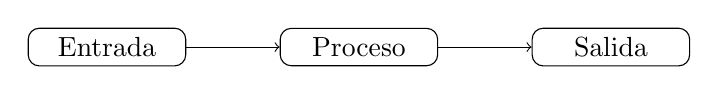
\begin{tikzpicture}[node distance=2.2cm, every node/.style={draw, rounded corners, minimum width=2cm}]
    \node (a) {Entrada};
    \node[right of=a, xshift=1cm] (b) {Proceso};
    \node[right of=b, xshift=1cm] (c) {Salida};
    \draw[->] (a) -- (b);
    \draw[->] (b) -- (c);
  \end{tikzpicture}
  \caption{Flujo del método.}
  \label{fig:flujo}
\end{figure}
\lipsum[19-24]
